
\documentclass[a4paper,10pt]{report}
\usepackage{blindtext} % for dummy texts
\usepackage[T1]{fontenc}
\usepackage[table]{xcolor}
\usepackage{titlesec}
\usepackage{graphicx}
%\usepackage[inkscapepath=../assets/svg]{svg}
\usepackage{amsmath}
\usepackage{amsthm}
\usepackage{amssymb}
\usepackage{mathtools}
\usepackage{fancyvrb}
\usepackage[english]{babel}
\usepackage{csquotes}
\usepackage{hyperref}
\usepackage{adjustbox,lipsum}
\hypersetup{
   colorlinks=true,
   linkcolor=blue,
   urlcolor=cyan
}
\usepackage{tikz}
\usepackage{amssymb}
\usepackage[sc]{mathpazo}
\linespread{1.05}
\usepackage{microtype}
\usepackage{breqn}
\usepackage{caption}
\usepackage{subcaption}
\usepackage[
   backend=bibtex,%
   bibencoding=utf8,%
   language=english,%
   style=numeric-comp,%
   sorting=nyt,%
   maxbibnames=10,%
   natbib=true%
]{biblatex}
\addbibresource{references.bib}
\usepackage{siunitx}
\usepackage{booktabs}
\usepackage{longtable}
\usepackage{geometry}
\usepackage{multirow}
\graphicspath{ {../assets/img/} }

\newgeometry{hmargin={30mm,30mm}}

% Set TOC depth and sections numbering
\setcounter{tocdepth}{3}
\setcounter{secnumdepth}{3}

% Remove chapters head and reduce spacing
\titleformat{\chapter}[hang]{\Large\bfseries}{\thechapter \hspace{2ex}}{0pt}{\Large}
\titlespacing{\chapter}{0cm}{0cm}{0.5cm}
\usepackage[parfill]{parskip}

% Make quotes italic
\renewcommand{\mkbegdispquote}[2]{\itshape}

% Change texttt line breaks
\renewcommand{\texttt}[1]{%
  \begingroup
  \ttfamily
  \begingroup\lccode`~=`.\lowercase{\endgroup\def~}{.\discretionary{}{}{}}%
  \catcode`/=\active\catcode`[=\active\catcode`.=\active
  \scantokens{#1\noexpand}%
  \endgroup
}

\titlespacing{\chapter}{0pt}{20pt}{0pt}


\begin{document}
\frenchspacing


%----------------------------------------------------------------------------------------
%	FIRST PAGE
%----------------------------------------------------------------------------------------
\title{
  {{\large{\textsc{Alma Mater Studiorum $\cdot$ University of Bologna}}}}
  \rule{\textwidth}{0.4pt}\vspace{3mm}
  \textbf{FantaBayesianNet\footnote{The code for the project is publicly available on \href{https://github.com/giuseppeboezio/FantaBayesianNet}{GitHub}}}
  \begin{figure}[!htb]
    \centering
    
\includegraphics[width = 100pt]{fantacalcio-icon}
  \end{figure} \\
  Fundamentals of Artificial Intelligence and Knowledge Representation (Module 3)
}

\author{ Giuseppe Murro (\href{mailto:giuseppe.murro@studio.unibo.it}{giuseppe.murro@studio.unibo.it}) \\ Giuseppe Boezio (\href{mailto:giuseppe.boezio@studio.unibo.it}{giuseppe.boezio@studio.unibo.it}) \\ Salvatore Pisciotta (\href{mailto:salvatore.pisciotta2@studio.unibo.it}{salvatore.pisciotta2@studio.unibo.it})}
\date{\today}
\maketitle
\newpage
\tableofcontents
\setcounter{tocdepth}{1}
%\listoffigures
%\listoftables
\newpage
%----------------------------------------------------------------------------------------



%----------------------------------------------------------------------------------------
%	INTRODUCTION
%----------------------------------------------------------------------------------------
\chapter{Introduction}\label{chap:introduction}

The task of predicting the performance of football players is gaining increasing attention in the sports and statistical communities. In this work, we used a Bayesian Network to model relevant factors of player performance in the presence of noisy data. We apply our analysis to the 2020–2021 season in the top Italian league, Serie A, and use the player ratings provided by a popular Italian fantasy football game, the so-called Fantacalcio.
Actually in literature there is a lack of published research on modeling this kind of data
within a Bayesian framework. The only work done on this field is \cite{bayesian_edigi_gabry} which propose various hierarchical models for predicting player ratings.

Instead in this project we are focused to explore the causal relations that allow to predict if a football player can be deployed or not in a fantasy football lineup. Different kind of reasoning are done to exploit the flow of influence between variables and possible independences. The implementation of the model and the methods used for inference are based on the pgmpy \cite{pgmpy} python library. 

%----------------------------------------------------------------------------------------




%----------------------------------------------------------------------------------------
%	BACKGROUND
%----------------------------------------------------------------------------------------
{\let\clearpage\relax\par \chapter{Background}\label{chap:background}} 


Fantasy sports games typically involve roster selection and match-by-match challenges against other participants with the results determined by the collective performance of the players on the fantasy rosters. In Italy, fantasy football was popularized by the brand \emph{Fantacalcio} \cite{fantacalcio} edited by Riccardo Albini in the 1990s and in the rest of the report we use the original denomination for referring at the Italian game.

Each player in the Italian Serie A league has an associated price determined by various factors including past performance and forecasts for the upcoming season.
At the beginning of the season, the virtual managers are allocated a limited amount of virtual money with which to buy the players that will comprise their roster. 
Each roster will consist of 3 goalkeepers, 8 defenders, 8 midfielders and 6 forwards.

For every matchday in Serie A, virtual managers must \textit{deploy} a fantasy team formed by 11 players divided into their respective roles according to the modules (often  4-3-3 or 3-4-3).
After every match, the prominent Italian sports periodicals assign each player a rating,
a so-called \textit{grade}, on a scale from 1 to 10. In practice there is not much variability in these grades; they typically range 4 four to 8, with the majority between 5 and 6. These grades are very general and largely subjective performance ratings that do not account for significant individual events (goals, assists, yellow and red cards, etc.) in a consistent way.

As a means of systematically including specific in-game events in the ratings, Fantacalcio provides the so-called \textit{point scoring system}. Points are added or deducted from a player’s initial grade for specific positive or negative events during the match. The point scores are more variable than the grades, especially across positions (e.g. when comparing defending and attacking players). Goalkeepers suffer the most from the point scoring system, as they are deducted a point for every goal conceded. On the other extreme,
forwards (attacking players) typically receive the highest point scores because every goal scored is worth three points.

For player \(i\) in match \(t\) the total score \(y_{i,t}\) is
\[y_{i,t} = G_{i,t} + P_{i,t}\]
where G is the grade and P is the point score. Table \ref{table:points} lists the game features that contribute to a player’s point score \(P_{i,t}\) for a given match. 


\begin{longtable}{m{0.3\linewidth}|m{0.3\linewidth}}
  \textbf{Event} & \textbf{Points} \\ \hline \endhead
    Goal             & +3       \\ 
    Assist           & +1       \\ 
    Penalty saved*  & +3       \\ \hline
    Yellow card      & -0.5     \\ 
    Red card         & -1       \\ 
    Goal conceded*   & -1       \\ 
    Own goal         & -2       \\ 
    Missed penalty  & -3       \\ \hline
    
  \caption{Bonus/Malus points in Fantacalcio. The symbol * denotes an event only applicable to goalkeepers.}
  \label{table:points}
\end{longtable}


Since it is very rare for a player to participate in all matches, some  \(y_{i,t}\) are missing, and this may be due to different reasons: 
\begin{itemize}
\item the player does not play in the match because of injury, disqualification, coach’s decision, or some other
reason;
\item the player does not participate in the match for long enough for their impact to
be judged by those tasked with assigning the subjective grade
\end{itemize}
For all these, the score is marked with the initials «sv».



%----------------------------------------------------------------------------------------


%----------------------------------------------------------------------------------------
%	CHAPTER 3
%----------------------------------------------------------------------------------------
{\let\clearpage\relax\par \chapter{Dataset}\label{chap:chapter-3}} 

\section{Data acquisition}\label{sec:sec-31}
The first step consists in load data, merge different data frames to get a single data frame of players and process feature in order to work with them.

Since statistics of single football players of Serie A in each mach are not directly accessible and they are distributed on different web sites, we have developed a web scraping script (accessible from the \href{https://github.com/giuseppeboezio/FantaBayesianNet/tree/main/src}{repository} of this project) able to collect data from \href{https://www.fantacalcio.it/statistiche-serie-a}{Fantacalcio.it} \cite{fantacalcio} and \href{https://www.transfermarkt.it/serie-a/startseite/wettbewerb/IT1}{Transfermarket.it} \cite{transfermarket} and merge them in order to obtain a single dataset.

We decided to select only forwards players, since their statistics are the most interesting from the view point of the Fantacalcio, and we picked an average of 2 players per team for a total amount of 40 players. 
These data are about the first 30 rounds of the 2020–2021 Serie A season.

\section{Data preprocessing}\label{sec:sec-32}
In the initial dataset we had a lot of data, but only some of them were useful for our model.
So starting from the raw dataset we applied three preprocessing operations:
\begin{itemize}
\item Data cleaning from useless columns and rows that refers to "postponed"  matches that did not have information about players, since the game was not played.
\item Data discretization since pgmpy does not support learning from continuous variable, and so all numerical values are mapped into bins
\item Data transformation of the missing values in the "score" attribute into the category "sv" (meaning without a score), which is the symbolic convention in Fantacalcio that indicates the absence of score for a player.
\end{itemize}


%----------------------------------------------------------------------------------------



%----------------------------------------------------------------------------------------
%	CHAPTER 4
%----------------------------------------------------------------------------------------
{\let\clearpage\relax\par \chapter{Bayesian network}\label{chap:chapter-4}}

\section{Structure}\label{sec:section-41}
\subsection{Variables}\label{subsec:subsection-411}
\begin{itemize}

    \item \textbf{goal} = Goal: represents whether, at the correspondent matchday, the player has made a goal and obtained the correspondent bonus (+3)
    \begin{itemize}
        \item True: the player has scored at least one goal
        \item False:The player didn't even score one goal
    \end{itemize}
    
    \item \textbf{assist} = Assist: represents whether, at the correspondent matchday, the player has made an assist and obtained the correspondent bonus (+3)
    \begin{itemize}
        \item True: The player has made at least one assist
        \item False:The player didn't even make one assist
    \end{itemize}
    
    \item \textbf{time_range} = Range of minutes: minutes played by the player in the correspondent match
    \begin{itemize}
        \item 0-15: The player played no more than 15 minutes
        \item 16-45:The player has played more than 15 minutes but less than 45 minutes
        \item 46-90:The player has played more than 45 minutes
    \end{itemize}
    
    \item \textbf{score_range} = Range of "fantasy score": fantasy score obtained by the player at the correspondent matchday, with appropriate bonus and malus included 
    \begin{itemize}
        \item s.v. :The player has not played or has played too little time to have a vote
        \item <=5 :the player had a bad game with some possible malus
        \item 5.5-6.5 :the player did not play a great game or at most a sufficient game
        \item 7-9.5 :the player played a great game and may have taken some bonuses as well
        \item >=10 :the player played an excellent game and also took some bonuses
    \end{itemize}
    
    \item \textbf{difficulty_match}= Difficulty of the match calculated in crescent order through a formula
    \begin{itemize}
        \item 1 :easy match generally played at home
        \item 2 :easy match generally played away
        \item 3 :balanced match
        \item 4 :difficult match generally played at home
        \item 5 :difficult match generally played away
    \end{itemize}
    
    \item \textbf{penalty_kicker}= Kicker of the team for penalties: represents whether the player (if at the correspondent matchday was available) is the one designed to kick the penalties
    \begin{itemize}
        \item True: The player is the penalty kicker
        \item False:The player isn't the penalty kicker
    \end{itemize}
    
    \item \textbf{home_match}= : represents whether, at the correspondent matchday, the player's team played at home or away
    \begin{itemize}
        \item True: the team played the match at home
        \item False: the team played the match away from home
     \end{itemize}
     
    \item \textbf{yellow_card}= Admonition: represents whether, at the correspondent matchday, the player the player got a yellow card with correspondent malus(-0.5)
    \begin{itemize}
        \item True: the player received a yellow card
        \item False: the player didn't receive a yellow card
    \end{itemize}
    
    \item \textbf{red_card}= Expulsion: represents whether, at the correspondent matchday, the player the player got a red card with correspondent malus(-1)
    \begin{itemize}
        \item True: the player received a red card
        \item False: the player didn't receive a red card
    \end{itemize}
    
    \item \textbf{available}= Availability: represent whether the player at the corresponding matchday was available for his team or not (e.g. for an injury or a disqualification)
    \begin{itemize}
        \item True: the player was available
        \item False: the player wasn't available
    \end{itemize}
    
    \item \textbf{deployability}=Deployability: represents whether the player for the corresponding matchday will be a good choice for the fantasy team of the fantasy manager
    \begin{itemize}
        \item True: deploy the player is a good choice
        \item False: it is better, if possible, not to deploy the player
    \end{itemize}
    
\end{itemize}

\newpage
\subsection{Network}\label{subsec:subsection-412}
The building step of the model started with the realization of the first network based only on the domain's knowledge. Move forward the structure was improved and developed using correlation matrix analysis that lead us to the final network presented in Figure \ref{fig:bayesianNet}.

\begin{figure}[h]
    \centering
    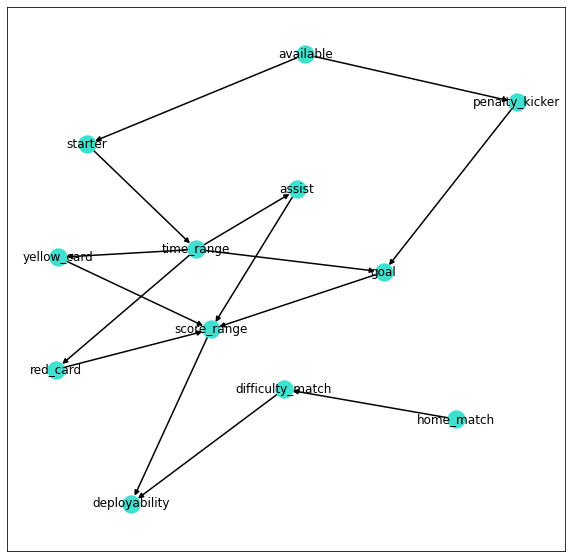
\includegraphics[width=0.5\textwidth]{assets/img/Network.png}
    \caption{Bayesian Network}
    \label{fig:bayesianNet}
\end{figure}



\section{Active Trails}\label{sec:section-42}
We have done some examples of reasoning patterns, namely causal reasoning and evidential reasoning, and possibile active-trails in the directed graph. A trail $X \leftrightharpoons Z \leftrightharpoons Y$ is active if influence can flow from $X$ to $Y$ via $Z$.

The first example consists in showing how \textbf{P(deployability)} is influenced by \textbf{available} because there is an active trail between the two variables and there is no evidence or V structure that can break it.

Then, it can be shown that \textbf{starter} in the evidence behaves as a blocking node breaking an active trail between the two aforementioned variables.

In both cases there is a flow of influence because the graph is \textbf{multiply connected} i.e. there is more than one trail which connects two nodes.\newline

Active trails are shown in figure \ref{fig:first_active_trail}

\begin{figure}[h]
    \centering
    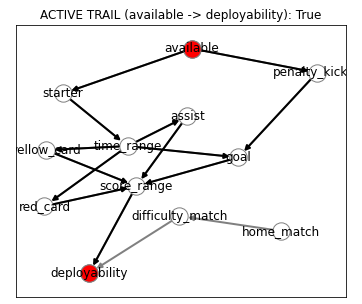
\includegraphics[width=0.45\textwidth]{assets/img/active_trail_1-1.PNG}
    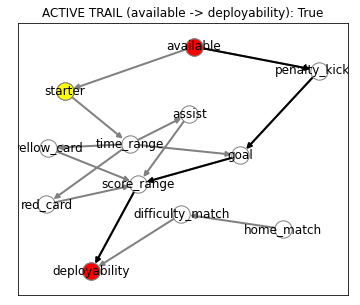
\includegraphics[width=0.45\textwidth]{assets/img/active_trail_1-2.PNG}
    \caption{Active trails between available and deployability}
    \label{fig:first_active_trail}
\end{figure}
\newpage

The second example consists in showing conditional independencies between variables: \textbf{starter} and \textbf{penalty_kicker} break the two possible active trails between \textbf{available} and \textbf{deployability}. This is compliant with the \textbf{d-separation principle}, that allows us to determine whether a set X of variables is independent of another set Y, given a third set Z: if there is no active trail between two variables X and Y, then X and Y are d-separated. Thus:

\begin{center}
    \[P \models (available \perp deployability|starter,penalty\_kicker)\]
\end{center}

This means that adding \textbf{available} to the evidence gives no additional information to the query. This can be proved also comparing the two probability distributions and showing that for all combinations of values they provide the same results.
Comparison is shown in figure \ref{fig:broken_trails}

\begin{figure}[h]
    \centering
    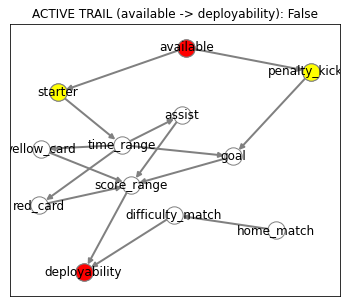
\includegraphics[width=0.45\textwidth]{assets/img/active_trail_2-1.PNG}
    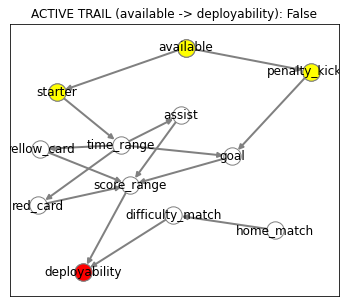
\includegraphics[width=0.45\textwidth]{assets/img/active_trail_2-2.PNG}
    \caption{Broken active trails}
    \label{fig:broken_trails}
\end{figure}


In the third example we are trying to understand whether a \textbf{score range} between 7-9.5 could be due to the fact that the player made a goal or not.

It can be shown also in this case that there is a \textbf{direct cause} from \textbf{goal} to \textbf{score_range}. This means that exists an active trail between the two variables.

Looking at the probability distribution, it can be understood how the goal could be a possible explanation to the received score with a probability around 58 \%.

The next step is to understand whether the goal could be a good explanation even if the player got a yellow card. In this case we put in the evidence also the \textbf{yellow card} and this variable influences the goal because \textbf{score_range} allows the activation of a V-structure, thus there is an active trail between \textbf{goal} and \textbf{yellow_card}.

An interesting thing is to highlight how the probability to have made a goal increases, probably because it is very difficult that a player can get a good score with a yellow card without a goal.
Active trail is shown in figure \ref{fig:active_with_V_structure}

\begin{figure}[h]
    \centering
    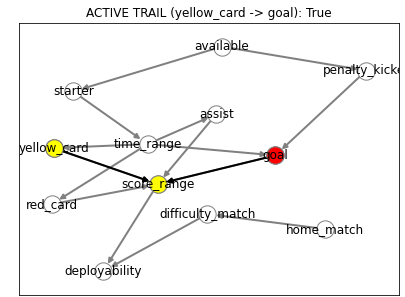
\includegraphics[width=0.70\textwidth]{assets/img/active_trail_3.PNG}
    \caption{Active trail with V structure}
    \label{fig:active_with_V_structure}
\end{figure}


\section{Independencies}\label{sec:section-43}

The V-structure between score_range and difficulty match allows to understand the independence between goal and difficulty match because this kind of structure breaks the only possible active trail between the two variables. In our domain this is quite reasonable becouse a good player can score a goal indipendetly by the opposing team. It has been shown in two different ways:
\begin{center}
    $P \models (goal \perp difficulty\_match)$
\end{center}

It has been shown in two different ways:
\begin{enumerate}
    \item Showing that \textbf{P(difficulty_match|goal) = P(difficulty_match)} as shown in figure \ref{fig:prob_distributions}
    \item Showing that there is no \textbf{active trail} in the graph between the two variables as showed in figure \ref{fig:independence}
\end{enumerate}

\begin{figure}[h]
  \centering\begin{minipage}[b]{0.45\textwidth}
    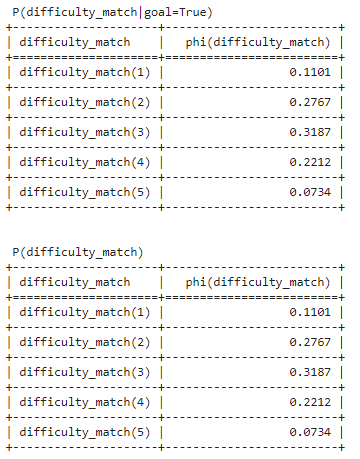
\includegraphics[width=\textwidth]{assets/img/prob_distributions.PNG}
\caption{Comparison between probability distributions}
\label{fig:prob_distributions}
  \end{minipage}
  \hfill\begin{minipage}[b]{0.45\textwidth}
    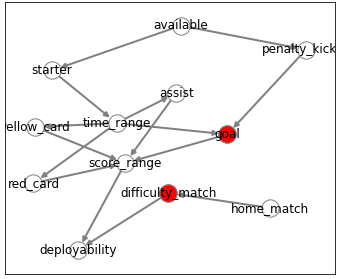
\includegraphics[width=\textwidth]{assets/img/Independence.PNG}
    \caption{Independence between goal and difficulty match}
\label{fig:independence}
  \end{minipage}
\end{figure}


%----------------------------------------------------------------------------------------


%----------------------------------------------------------------------------------------
%	CHAPTER 5
%----------------------------------------------------------------------------------------
\chapter{Inference}\label{chap:chapter-5}

\section{Exact Inference}\label{sec:section-51}

The query considered for a deeper analysis with exact inference is the probability of the player to be deployed given that he is a starter, more formally

\[ P(Deployability|starter) \]

There are different ways to solve with exact inference this query.
The first method, which is not the best one, consists of using marginalization property and global semantics to decompose the probability as the product of different probabilities iterating over the variables which are neither query variables nor evidence ones. This method is called inference by enumeration.
For previous query write the whole decomposition would be too chaotic and dispersive, thus it will be provided a sketch of the steps to follow

\[ \alpha P(Deployability,starter) \]

\[ \alpha \sum_{hidden} P(Deployability,starter, hidden) \]

\[ \alpha \sum_{hidden} P(Deployability|difficulty \,match, score\, range) P(starter|available)P(hidden|parents(hidden)) \]

The query is solved using a depth first search which turns out to be not so efficient because same terms appearing in different branches are computed several times.

Better results can be obtained using a sort of dynamic programming which allows to store intermediate results avoiding repeated calculations. There are different methods in this category, the one that has been used to execute the query is called variable elimination and consists of the following steps:

\begin{itemize}
    \item substituting each probability in the first formula with a factor which is a matrix built considering variables over which there is the summation. For example:
    
    \[ P(Deployability|difficulty\,match,score\,range) \]
    
    will become $f_n(Deployability, Difficulty\,match, Score\,range)$
    
    \item Then, in right-to-left order factors are multiplied (element-wise) getting new simplified factors which allow to get an intermediate result and saving time and space for computations.
    
\end{itemize}

Different ordering of the variables can be tried but as heuristic a good one consists of eliminating whichever variable minimizes the size of the next factor to be constructed.
It means to eliminate all variables which are ancestors neither the query variable nor evidence ones nor d-separated from both of them.\newline\newline
In our query there are not variables that can be eliminated because starting from deployability it is possible to reach all ancestors.
\newline

Variable elimination algorithm can be executed using different heuristics to order elimination variables. Heuristics adopted in pgmpy are the followings:

\begin{itemize}
    \item MinFill: the number of edges that need to be added to the graph due to its elimination.
    \item MinNeighbors: the number of neighbors it has in the current graph.
    \item MinWeight: the product of weights, domain cardinality, of its neighbors.
    \item WeightedMinFill: the sum of weights of the edges that need to be added to the graph due to its elimination, where a weight of an edge is the product of the weights, domain cardinality, of its constituent vertices.
\end{itemize}

Considering the query:

\begin{center}
    $P(deployability|starter=True)$
\end{center}

it can be shown that query results using previously mentioned heuristics are the same but we have better time performance using MinWeight.

Following table shows different results and orderings.\newline

\adjustbox{max width=\columnwidth}{
 \begin{tabular}{||c c c ||} 
 \hline
 Heuristic & Ordering & Time \\ [0.5ex] 
 \hline\hline
 MinFill & [red_card, score_range, home_match, difficulty_match, goal, yellow_card, time_range, penalty_kicker, available, assist] & 0.068 s \\ 
 \hline
 MinNeighbors & [home_match, available, difficulty_match, penalty_kicker, red_card, time_range, goal, yellow_card, assist, score_range] & 0.035 s \\
 \hline
 MinWeight & [available, home_match, penalty_kicker, difficulty_match, time_range, score_range, red_card, goal, yellow_card, assist]	 & 0.031 s\\
 \hline
 WeightedMinFill & [home_match, available, penalty_kicker, difficulty_match, time_range, score_range, red_card, goal, yellow_card, assist] & 0.034 s \\ [1ex] 
 \hline
\end{tabular}
}

A problem of exact inference with variable elimination is that it is NP-hard in the case of multiply connected networks (i.e. there are multiple trails to connect two variables) as the network of this project.


\section{Approximate Inference}\label{sec:section-52}
Starting from the results provided by the exact inference, using the variable elimination method, it is possible to analyze and compare the behavior of three approximate inference methods: the rejection sampling, the likelihood weighting and the Gibbs sampling all of them implemented using the pgmpy library.


To observe how these inference methods behave in different situations, we tested 4 interesting queries:

\begin{enumerate}
    \item$P(goal|assist )$
    \newline
    The result of this query (see Fig. \ref{fig:query1results}) highlights that a player has a probability of around 30\% of make goal when he has already done an assist. Starting from the fact that the probability of a player to score a goal, without any evidence, is around 25\% we can deduce that the probability increase due to the more comfortable approach of the forward into the match.
          

    \item $P(penalty\_kicker\ | available, goal,\neg starter)$
    \newline
    This query shows (see Fig. \ref{fig:query2results}) that whether a player scored a goal starting the match from the bench, there is a probability of 53\% that he is the penalty kicker of the team. This result highlights that it is quite probable that the goal is the consequence of a marked penalty.
\end{enumerate}
    \textbf{Analysis of sampling methods:}
        \newline
        As we can see from \ref{fig:query1results} and \ref{fig:query2results} since the second query has more evidence of the first one the time of the rejection sampling dramatically increase. On the contrary, likelihood weighting and Gibbs sampling maintain the same sampling times. Indeed, the method of rejection sampling is implemented by generating samples from forward sampling and rejects those that do not match our evidence and keep doing until it has as sample as the sample size.
        Moreover, Gibbs sampling appears poorly when the sample sizes are not big. This is due to the implementation of the sampling method in pgmpy library since it does not allow to explicit the evidence variables. For this reason, a lot of samples that are not compatible with evidence are rejected.

    \begin{figure}[h]
      \centering\begin{minipage}[b]{0.45\textwidth}
        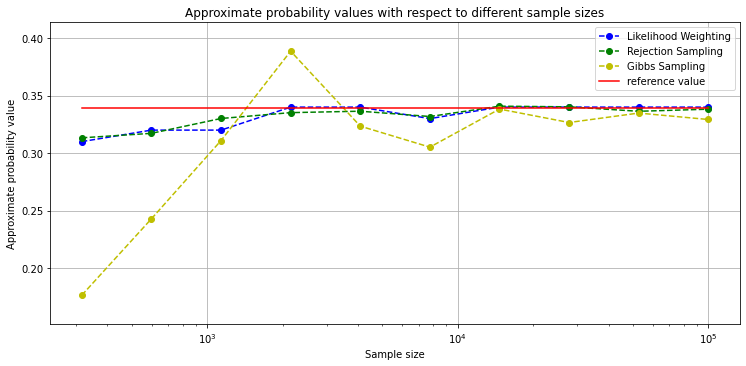
\includegraphics[width=\textwidth]{assets/img/query1prob.png}
      \end{minipage}
      \hfill\begin{minipage}[b]{0.45\textwidth}
        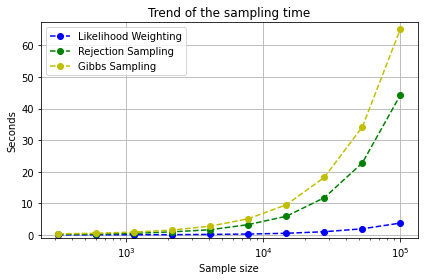
\includegraphics[width=\textwidth]{assets/img/query1time.png}
      \end{minipage}
    \caption{Probability values and sampling times of $P(goal|assist )$}
    \label{fig:query1results}
    \end{figure}
    
    \begin{figure}[h]
      \centering\begin{minipage}[b]{0.45\textwidth}
        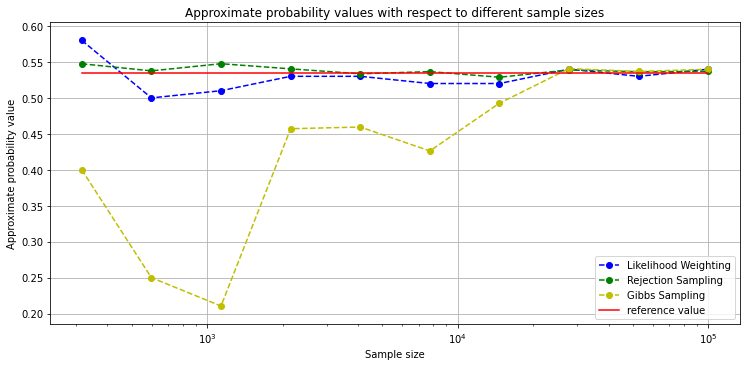
\includegraphics[width=\textwidth]{assets/img/query2prob.png}
      \end{minipage}
      \hfill\begin{minipage}[b]{0.45\textwidth}
        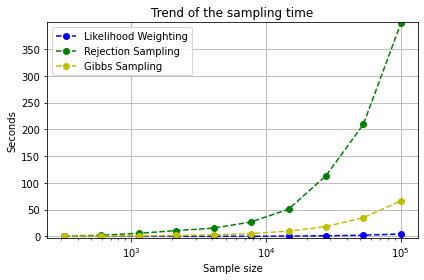
\includegraphics[width=\textwidth]{assets/img/query2time.png}
      \end{minipage}
    \caption{Probability values and sampling times of $P(penalty\_kicker | available, goal,\neg starter)$}
    \label{fig:query2results}
    \end{figure}

\begin{enumerate}
\addtocounter{enumi}{2}
    \item$P(deployability | yellow\_card, assist)$
    \newline
  The result of the query it is quite interesting because the malus of the yellow card (-0.5) doesn't influence the deployability. This happens because, nevertheless the player has received an admonition he played a good game with an assist (bonus +1), so it is a good choice to deploy him in lineup.
          

    \item $P(goal | time\_range = 0-15)$
    \newline
    The result of this query is quite obvious, a player need more minutes to score a goal, so if you are looking for a high score in your Fantacalcio team and you know that the forward could play only few minutes, it is better not to deploy him.
\end{enumerate}

\textbf{Analysis of sampling methods:}
    \newline
    As we can see from \ref{fig:query3results} and \ref{fig:query4results} the errors of likelihood weighting and Gibbs sampling are higher in these two queries with respect to previous two. This happens because they converge really slow with probabilities close to 0 (like in the forth query) and 1 (like in the third query)

\begin{figure}[h]
  \centering\begin{minipage}[b]{0.45\textwidth}
    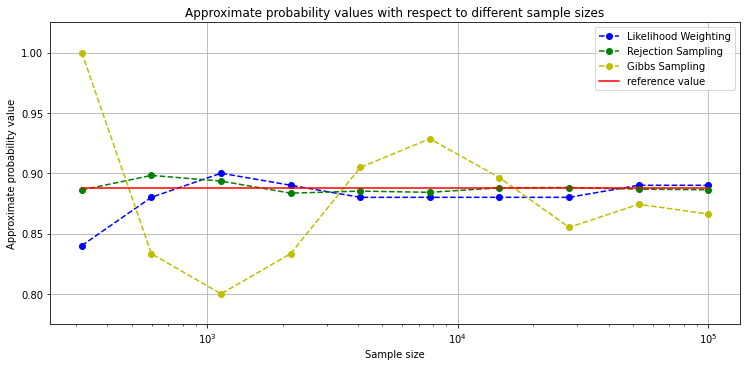
\includegraphics[width=\textwidth]{assets/img/query3prob.png}
  \end{minipage}
  \hfill\begin{minipage}[b]{0.45\textwidth}
    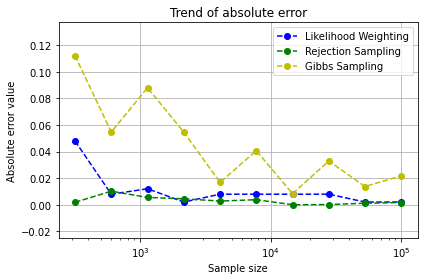
\includegraphics[width=\textwidth]{assets/img/query3error.png}
  \end{minipage}
\caption{Probability values and absolute error trend of $P(deployability | yellow\_card, assist)$}
\label{fig:query3results}
\end{figure}

\begin{figure}[h]
  \centering\begin{minipage}[b]{0.45\textwidth}
    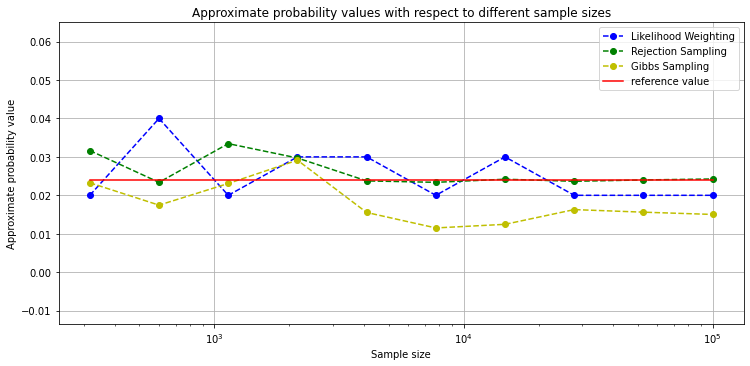
\includegraphics[width=\textwidth]{assets/img/query4prob.png}
  \end{minipage}
  \hfill\begin{minipage}[b]{0.45\textwidth}
    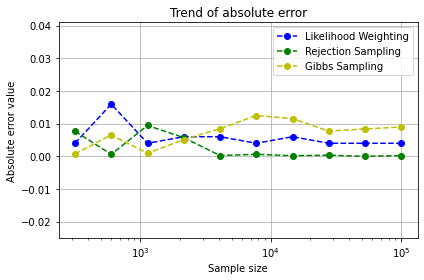
\includegraphics[width=\textwidth]{assets/img/query4error.png}
  \end{minipage}
\caption{Probability values absolute error trend of $P(goal | time\_range = 0-15)$}
\label{fig:query4results}
\end{figure}

%----------------------------------------------------------------------------------------



%----------------------------------------------------------------------------------------
%	CHAPTER 6
%----------------------------------------------------------------------------------------
\chapter{Conclusion and future works}\label{chap:chapter}
The results provided in this paper are reasonable admissible but since we tried to make inference about a complete stochastic domain, it found out to be really difficult to obtain good results because it was not always possible to take into account the enormous amount of variables that effectively affect the domain of our analysis and construct a model on it.
A possible different analysis based on our model could be to extend the dataset of players, considering not only forwards but also midfielders and defenders in order to prove whether the model could be a good base to develop a real software that helps fantasy managers to solve their doubts in line up their fantasy football formation.


%----------------------------------------------------------------------------------------


%----------------------------------------------------------------------------------------
%	REFERENCES
%----------------------------------------------------------------------------------------
{\let\clearpage\relax\par \printbibliography}

\end{document}
